\documentclass[12pt,]{article}
\usepackage{lmodern}
\usepackage{amssymb,amsmath}
\usepackage{ifxetex,ifluatex}
\usepackage{fixltx2e} % provides \textsubscript
\ifnum 0\ifxetex 1\fi\ifluatex 1\fi=0 % if pdftex
  \usepackage[T1]{fontenc}
  \usepackage[utf8]{inputenc}
\else % if luatex or xelatex
  \ifxetex
    \usepackage{mathspec}
  \else
    \usepackage{fontspec}
  \fi
  \defaultfontfeatures{Ligatures=TeX,Scale=MatchLowercase}
\fi
% use upquote if available, for straight quotes in verbatim environments
\IfFileExists{upquote.sty}{\usepackage{upquote}}{}
% use microtype if available
\IfFileExists{microtype.sty}{%
\usepackage{microtype}
\UseMicrotypeSet[protrusion]{basicmath} % disable protrusion for tt fonts
}{}
\usepackage[margin=1in]{geometry}
\usepackage{hyperref}
\PassOptionsToPackage{usenames,dvipsnames}{color} % color is loaded by hyperref
\hypersetup{unicode=true,
            colorlinks=true,
            linkcolor=black,
            citecolor=Blue,
            urlcolor=black,
            breaklinks=true}
\urlstyle{same}  % don't use monospace font for urls
\usepackage{longtable,booktabs}
\usepackage{graphicx,grffile}
\makeatletter
\def\maxwidth{\ifdim\Gin@nat@width>\linewidth\linewidth\else\Gin@nat@width\fi}
\def\maxheight{\ifdim\Gin@nat@height>\textheight\textheight\else\Gin@nat@height\fi}
\makeatother
% Scale images if necessary, so that they will not overflow the page
% margins by default, and it is still possible to overwrite the defaults
% using explicit options in \includegraphics[width, height, ...]{}
\setkeys{Gin}{width=\maxwidth,height=\maxheight,keepaspectratio}
\IfFileExists{parskip.sty}{%
\usepackage{parskip}
}{% else
\setlength{\parindent}{0pt}
\setlength{\parskip}{6pt plus 2pt minus 1pt}
}
\setlength{\emergencystretch}{3em}  % prevent overfull lines
\providecommand{\tightlist}{%
  \setlength{\itemsep}{0pt}\setlength{\parskip}{0pt}}
\setcounter{secnumdepth}{5}

%%% Use protect on footnotes to avoid problems with footnotes in titles
\let\rmarkdownfootnote\footnote%
\def\footnote{\protect\rmarkdownfootnote}

%%% Change title format to be more compact
\usepackage{titling}

% Create subtitle command for use in maketitle
\newcommand{\subtitle}[1]{
  \posttitle{
    \begin{center}\large#1\end{center}
    }
}

\setlength{\droptitle}{-2em}
  \title{}
  \pretitle{\vspace{\droptitle}}
  \posttitle{}
  \author{}
  \preauthor{}\postauthor{}
  \date{}
  \predate{}\postdate{}

\usepackage{amsmath}
\usepackage{setspace}
\usepackage{rotating}
\usepackage[dvipsnames]{xcolor}
\usepackage{tgtermes}
\definecolor{mycol}{gray}{0.1}
\color{mycol}
\usepackage{enumitem}
\usepackage{wrapfig}
\usepackage[font={footnotesize,it}]{caption}
\usepackage{floatrow}
\usepackage{mathptmx}
\usepackage{titlesec}
\titleformat{\section}{\normalfont\fontsize{14}{15}\bfseries}{\thesection}{1 em}{}
\titleformat{\subsection}{\normalfont\fontsize{12}{15}\bfseries}{\thesubsection}{1 em}{}
\titlespacing{\section}{0pt}{\parskip}{-\lineskip}
\titlespacing{\subsection}{0pt}{\parskip}{-\parskip}
\titlespacing{\subsubsection}{0pt}{\parskip}{-\parskip}

\begin{document}

\pagenumbering{roman}

\begin{description}
\item[Date:] \today
\item[Descriptive Title:] Synthesizing time series of plant and animal populations to understand the limits to ecological forecasts
\item[Short Title:] Ecological Forecasting
\item[PI Contact Information:] ~\\
\vspace{-1.5em}
\begin{description}
 \item[\textcolor{mycol}{Andrew Tredennick}] (atredenn@gmail.com; 970-443-1599) \\ Utah State University \\ 5230 Old Main Hill, Logan, UT 84332
 \item[\textcolor{mycol}{Mevin Hooten}] (Mevin.Hooten@colostate.edu) \\ United States Geological Survey \\ Colorado State University \\ Fort Collins, CO 80523
 \item[\textcolor{mycol}{Peter Adler}] (peter.adler@usu.edu) \\ Utah State University \\ 5230 Old Main Hill, Logan, UT 84332
\end{description}
\item[Project Summary:] Forecasting the impacts of global environmental change is a major challenge facing ecologists and land managers in the 21\textsuperscript{st} century. Unfortunately, our knowledge of the limits to ecological forecasts lags behind our deep understanding of ecological systems. Fortunately, emerging theory on partitioning forecast uncertainty provides an opportunity to better understand the limits to ecological forecasts. We propose to convene a diverse working group of quantitative ecologists, each with detailed knowledge of a particular study system, to develop forecasting models of plant and animal populations. As a team, we will partition the forecast uncertainty for each focal population to test fundamental hypotheses about the relationship between particular sources of uncertainty and ecological characteristics. We will develop a forecast repository and a synthetic database of population time series coupled with environmental covariates that will be ideal for teaching and research. We anticipate our work will catalyze a new research area in ecology focused on identifying the boundaries of ecological forecasts based on ecological theory. 
\item[Proposed Start and End Dates:] October 2017 to September 2019, with two 4-day meetings at the Powell Center
\item[Proposed Data Release Date:] September 2019
\item[Total Requested Budget:] \$130,801 (Year 1 \$23,565; Year 2 \$107,236)
\item[Is this a resubmission?] No
\item[Conflicts of Interest with Reviewers:] None
\item[Keywords:] climate and land use change; ecosystems
\end{description}

\newpage{}

\pagenumbering{arabic}

\section{Problem Statement}\vspace{-1em}

\small{}
\phantom{}\hspace{8em}\textit{``...ecologists do not predict because when we do it reveals how little\\\phantom{}\hspace{8em}we understand about the natural world.''}
--\textit{Houlahan et al. 2017}

\normalsize{} \vspace{0.5em} A fundamental challenge facing society is
to predict the ecological impacts of global environmental changes such
as nitrogen deposition, climate change, and habitat fragmentation. Each
of these global change drivers have now exceeded their historical ranges
of variability (Steffen et al. 2015), meaning we are entering a
no-analog world in which we can no longer look to the past to predict
the future. We can, however, look to the past to parameterize models
that allow us to \emph{forecast} the future states of ecological systems
(Clark et al. 2001). Ecologists are in an excellent position to meet
this forecasting challenge because we have spent decades gaining
understanding of the processes that regulate populations, communities,
and ecosystems. However, we lack a systematic understanding of the
current limits to ecological forecasts. As a result, we do not know how
to allocate research effort to improve our forecasts.

Making poor forecasts is inevitable as ecology matures into a more
predictive science. The key is to learn from our failures so that
forecasts become more accurate over time. The success of meteorological
forecasting tells us that basic research on the causes of forecast
uncertainty is essential (Bauer et al. 2015). In ecology, a powerful
approach is to combine our detailed knowledge of organisms and ecosystem
processes with emerging knowledge on forecast uncertainty (Petchey et
al. 2015).

Dietze (2017) proposed a first-principles approach to partitioning
forecast uncertainty. Consider a dynamical model designed to predict
some state \emph{y} in the future (\(y_{t+1}\)) based on the current
state (\(y_{t}\)), an environmental driver(s) (\(x\)), parameters
(\(\theta\)), and process error (\(\epsilon\)). We can then write a
general form of the model as: \vspace{-2em}

\begin{align}
y_{t+1} = f(y_t, x_t|\theta) + \epsilon,
\end{align}\vspace{-2em}

which states that \(y\) at time \(t+1\) is a function of \(y\) and \(x\)
at time \(t\) conditional on the model parameters (\(\theta\)) plus
process error (\(\epsilon\)).
Dietze (2017) showed that forecast variance (\(Var[y_{t+1}]\)) is:
\vspace{-1em}

\begin{align}
Var[y_{t+1}] = \underbrace{\left(\frac{\delta f}{\delta y} \right)^2}_{\text{stability}} 
               \underbrace{\vphantom{ \left(\frac{\delta f}{\delta y} \right)^2 } Var[y_t]}_{\text{IC uncert.}} +
               \underbrace{\vphantom{ \left(\frac{\delta f}{\delta y} \right)^2 }\left(\frac{\delta f}{\delta x} \right)^2}_{\text{driver sens.}} 
               \underbrace{\vphantom{ \left(\frac{\delta f}{\delta y} \right)^2 } Var[x_t]}_{\text{driver uncert.}} +
               \underbrace{\vphantom{ \left(\frac{\delta f}{\delta y} \right)^2 }\left(\frac{\delta f}{\delta \theta} \right)^2}_{\text{param sens.}}
               \underbrace{\vphantom{ \left(\frac{\delta f}{\delta y} \right)^2 } Var[\theta]}_{\text{param. uncert.}} +
               \underbrace{\vphantom{ \left(\frac{\delta f}{\delta y} \right)^2 } Var[\epsilon]}_{\text{process error}},
\end{align}\vspace{-1em}

where each additive term follows a pattern of \emph{sensitivity} times
\emph{variance} (``IC uncert.'' refers to ``\emph{I}nitial
\emph{C}onditions uncertainty''). The variance attributable to any
particular factor is a function of how sensitive the model is to the
factor and the variance of that factor. For example, large sensitivity
to the covariate \(x\) can be offset if the uncertainty of the covariate
is low. Knowing the relative size of these uncertainties is important to
guide future research on ecological processes, data collection schemes,
and the application of forecasting models to applied questions. 
Understanding how sources of forecast uncertainty
systematically covary with ecological characteristics will allow us to
identify the potential limits to forecasts based on ecological theory.

The goal of this project is to synthesize forecasts of plant and animal
populations to advance our fundamental knowledge of the limits to
ecological forecasts. We will convene a diverse group of population
ecologists to partition forecast uncertainty for several species and
systematically link sources of uncertainty to characteristics of the
focal populations (e.g., life history traits).

\section{Hypotheses}

All forecasts are uncertain, and reducing forecast uncertainty hinges
upon knowing the source of uncertainty. The premise of this proposal is
that ecological characteristics of organisms (e.g., life history) are
related to sources of forecast uncertainty. Specifically, we pose three
hypotheses motivated by recent reviews of ecological forecasting
(Petchey et al. 2015; Houlahan et al. 2017).

\begin{description}

\item[H1.] \textbf{The contribution of initial conditions uncertainty to forecast uncertainty is greater for fast growing populations than for slow growing populations.} Fast growing populations are more likely to exhibit chaotic or near-chaotic dynamics, which inflate forecast uncertainty due to initial conditions uncertainty. To test this hypothesis we will partition forecasts and regress the proportion of uncertainty attributable to initial conditions against estimated intrinsic population growth rates.

\item[H2.] \textbf{The contribution of driver uncertainty to forecast uncertainty is greater for species that ``predict'' than for species that ``bet-hedge'' against environmental conditions.} In variable environments, annual plants have developed two main strategies for maintaining fitness despite changing conditions: (i) bet-hedging, where germination is low but constant, and (ii) predictive germination, where germination rates, cued by the environment, vary substantially from year to year. Bet-hedgers should be insensitive to environmental drivers, so their forecast uncertainties should not be driven by driver uncertainty. We will compare forecast partitions for winter annual plants that span a spectrum from bet-hedgers to predictors (Gremer et al. 2014) to test this hypothesis. We also anticipate applying this approach to our other focal data sets by quantifying variation of annual vital rates to determine where species lie on the bet-hedging spectrum (e.g., Botero et al. 2015).

\item[H3.] \textbf{The contribution of process uncertainty to forecast uncertainty increases with the number of trophic links.} We are using single-species population models in which trophic interactions are implicit, not explicit. Therefore, if trophic interactions are important our models will poorly represent the process. We will compare forecast partitions for all data sets to test this hypothesis. Our working group will consist of experts for each data set (Tables 1 and 2), meaning we will be able to develop food webs for each focal species based on expert knowledge. We recognize that constructing subjective food webs is a coarse approach, but in practice our knowledge of a species' trophic connections is typically coarse. Thus, we contend that our proposed approach is actually well-suited to addressing the practical challenge of linking forecast uncertainty to trophic connections.

\end{description}

Testing our hypotheses requires applying a standardized analytical approach to
a synthetic data set representative of many species -- an activity that can only
be done at the Powell Center as a working group.
These three hypotheses are just a starting point,
as the working group will generate additional hypotheses.

\section{Proposed Activities}

PIs Tredennick, Hooten, and Adler have led several efforts to forecast
the response of plant populations to climate change (Tredennick et al.
2016a, 2016b). Our frustration with the high levels of uncertainty in
our forecasts, and our inability to attribute that uncertainty to
specific causes, has motivated this proposal. We seek to (1) assemble a
database of publicly available time series of plant and animal
abundances which contain the necessary data, (2) use those data to fit
forecasting models, and (3) partition the forecast uncertainty from
those models to better understand the limits to ecological forecasting.
We have learned that collating large data sets and rigorously fitting
statistical population models requires dedicated effort. We therefore
request funding for a Powell Fellow (PI Tredennick) to lead all aspects
of our proposed work.

\subsection{Data Synthesis}
We have identified several potential data
sets (Table 1) and we anticipate our working group members (Table 2)
will be able to identify more based on their professional networks. One of our first tasks as a working group will be to develop
a set of criteria for selecting data. These criteria will include, but
are not limited to, cut-offs for length of time series, availability of suitable climate and other
environmental data, and the number of replicate observations within a
time period. Our goal is to assemble a database with equal
representation of plant and animal species.

The assembled database will contain yearly abundance estimates coupled
with environmental covariates, setting it apart from other population
time series that do not include potential drivers (e.g., Global
Population Dynamics Database). 
 All abundance data sets will
be combined into a single database that can be queried using standard
SQL software. The abundance data will be linked to a
second database of environmental
covariates. We will extract climate
data as needed from gridded data products (e.g., PRISM). We will work with study
area experts (Table 2) to decide on
appropriate climate covariates for each time series. This is
a preliminary data processing workflow; we will work with Powell Center experts to synthesize our data sets.

\footnotesize

\begin{longtable}[]{@{}llll@{}}
\caption{Publicly-available abundance time series for plants and
animals.}\tabularnewline
\toprule
\begin{minipage}[b]{0.06\columnwidth}\raggedright\strut
Taxa\strut
\end{minipage} & \begin{minipage}[b]{0.32\columnwidth}\raggedright\strut
Species (common name)\strut
\end{minipage} & \begin{minipage}[b]{0.22\columnwidth}\raggedright\strut
Length (yrs.)\strut
\end{minipage} & \begin{minipage}[b]{0.28\columnwidth}\raggedright\strut
Citation/Website\strut
\end{minipage}\tabularnewline
\midrule
\endfirsthead
\toprule
\begin{minipage}[b]{0.06\columnwidth}\raggedright\strut
Taxa\strut
\end{minipage} & \begin{minipage}[b]{0.32\columnwidth}\raggedright\strut
Species (common name)\strut
\end{minipage} & \begin{minipage}[b]{0.22\columnwidth}\raggedright\strut
Length (yrs.)\strut
\end{minipage} & \begin{minipage}[b]{0.28\columnwidth}\raggedright\strut
Citation/Website\strut
\end{minipage}\tabularnewline
\midrule
\endhead
\begin{minipage}[t]{0.06\columnwidth}\raggedright\strut
Animal\strut
\end{minipage} & \begin{minipage}[t]{0.32\columnwidth}\raggedright\strut
\emph{Bison bison} (American Bison)\strut
\end{minipage} & \begin{minipage}[t]{0.22\columnwidth}\raggedright\strut
35\strut
\end{minipage} & \begin{minipage}[t]{0.28\columnwidth}\raggedright\strut
Hobbs et al. (2015)\strut
\end{minipage}\tabularnewline
\begin{minipage}[t]{0.06\columnwidth}\raggedright\strut
Animal\strut
\end{minipage} & \begin{minipage}[t]{0.32\columnwidth}\raggedright\strut
\emph{Enhydra lutris} (Sea otter)\strut
\end{minipage} & \begin{minipage}[t]{0.22\columnwidth}\raggedright\strut
20\strut
\end{minipage} & \begin{minipage}[t]{0.28\columnwidth}\raggedright\strut
Williams et al. (2017)\strut
\end{minipage}\tabularnewline
\begin{minipage}[t]{0.06\columnwidth}\raggedright\strut
Animal\strut
\end{minipage} & \begin{minipage}[t]{0.32\columnwidth}\raggedright\strut
Breeding birds*\strut
\end{minipage} & \begin{minipage}[t]{0.22\columnwidth}\raggedright\strut
47\strut
\end{minipage} & \begin{minipage}[t]{0.28\columnwidth}\raggedright\strut
\url{http://www.pwrc.usgs.gov/bbs/}\strut
\end{minipage}\tabularnewline
\begin{minipage}[t]{0.06\columnwidth}\raggedright\strut
Animal\strut
\end{minipage} & \begin{minipage}[t]{0.32\columnwidth}\raggedright\strut
\emph{Dipodomys} spp. (Kangaroo rats)*\strut
\end{minipage} & \begin{minipage}[t]{0.22\columnwidth}\raggedright\strut
39\strut
\end{minipage} & \begin{minipage}[t]{0.28\columnwidth}\raggedright\strut
Ernest et al. (2015)\strut
\end{minipage}\tabularnewline
\begin{minipage}[t]{0.06\columnwidth}\raggedright\strut
Animal\strut
\end{minipage} & \begin{minipage}[t]{0.32\columnwidth}\raggedright\strut
Grasshopper spp.*\strut
\end{minipage} & \begin{minipage}[t]{0.22\columnwidth}\raggedright\strut
10 (with weekly census)\strut
\end{minipage} & \begin{minipage}[t]{0.28\columnwidth}\raggedright\strut
\url{http://ghopclimate.colorado.edu}\strut
\end{minipage}\tabularnewline
\begin{minipage}[t]{0.06\columnwidth}\raggedright\strut
Plant\strut
\end{minipage} & \begin{minipage}[t]{0.32\columnwidth}\raggedright\strut
Sagebrush steppe perennial plants*\strut
\end{minipage} & \begin{minipage}[t]{0.22\columnwidth}\raggedright\strut
22\strut
\end{minipage} & \begin{minipage}[t]{0.28\columnwidth}\raggedright\strut
Zachmann et al. (2010)\strut
\end{minipage}\tabularnewline
\begin{minipage}[t]{0.06\columnwidth}\raggedright\strut
Plant\strut
\end{minipage} & \begin{minipage}[t]{0.32\columnwidth}\raggedright\strut
AZ desert annuals*\strut
\end{minipage} & \begin{minipage}[t]{0.22\columnwidth}\raggedright\strut
14\strut
\end{minipage} & \begin{minipage}[t]{0.28\columnwidth}\raggedright\strut
Ernest et al. (2015)\strut
\end{minipage}\tabularnewline
\begin{minipage}[t]{0.06\columnwidth}\raggedright\strut
Plant\strut
\end{minipage} & \begin{minipage}[t]{0.32\columnwidth}\raggedright\strut
\emph{Artemisia} spp. (Sagebrush spp.)\strut
\end{minipage} & \begin{minipage}[t]{0.22\columnwidth}\raggedright\strut
27\strut
\end{minipage} & \begin{minipage}[t]{0.28\columnwidth}\raggedright\strut
Homer et al. (2013)\strut
\end{minipage}\tabularnewline
\begin{minipage}[t]{0.06\columnwidth}\raggedright\strut
Plant\strut
\end{minipage} & \begin{minipage}[t]{0.32\columnwidth}\raggedright\strut
Alpine tundra plants*\strut
\end{minipage} & \begin{minipage}[t]{0.22\columnwidth}\raggedright\strut
11\strut
\end{minipage} & \begin{minipage}[t]{0.28\columnwidth}\raggedright\strut
\url{http://niwot.colorado.edu/}\strut
\end{minipage}\tabularnewline
\begin{minipage}[t]{0.06\columnwidth}\raggedright\strut
Plant\strut
\end{minipage} & \begin{minipage}[t]{0.32\columnwidth}\raggedright\strut
Winter annuals (Desert Lab LTREB)*\strut
\end{minipage} & \begin{minipage}[t]{0.22\columnwidth}\raggedright\strut
30\strut
\end{minipage} & \begin{minipage}[t]{0.28\columnwidth}\raggedright\strut
Gremer and Venable (2014)\strut
\end{minipage}\tabularnewline
\begin{minipage}[t]{0.06\columnwidth}\raggedright\strut
Plant\strut
\end{minipage} & \begin{minipage}[t]{0.32\columnwidth}\raggedright\strut
Mt. St.~Helens plants*\strut
\end{minipage} & \begin{minipage}[t]{0.22\columnwidth}\raggedright\strut
30\strut
\end{minipage} & \begin{minipage}[t]{0.28\columnwidth}\raggedright\strut
del Moral (2010)\strut
\end{minipage}\tabularnewline
\bottomrule
\end{longtable}

\vspace{-2em}

*These data sets contain observations for many species.

\normalsize

\subsection{Analysis}\subsubsection{Dynamic Forecasting Models}

Using the assembled abundance time series, we will fit
Bayesian hierarchical state-space models, which are
well-suited for ecological forecasting because they inherently
incorporate and propagate the sources of uncertainty we seek to
partition: process uncertainty, observation uncertainty, and parameter
uncertainty. State-space models also explicitly acknowledge that our
observations are imperfect, meaning that the state we want to estimate
(e.g., abundance of bison in Yellowstone) is unknowable,
or \emph{latent}. A typical state-space model takes the form:
\vspace{-2em}

\begin{align}
y_t &\sim \text{Normal}(z_t, \sigma_{obs.}) \\
z_t &\sim \text{Normal}(\mu_t, \sigma_{proc.}) \\
\mu_t &= f(\boldsymbol{\theta_p},z_{t-1},\bold{x}),
\end{align}\vspace{-2em}

\begin{wrapfigure}[30]{r}{0.45\textwidth}
  \centering
     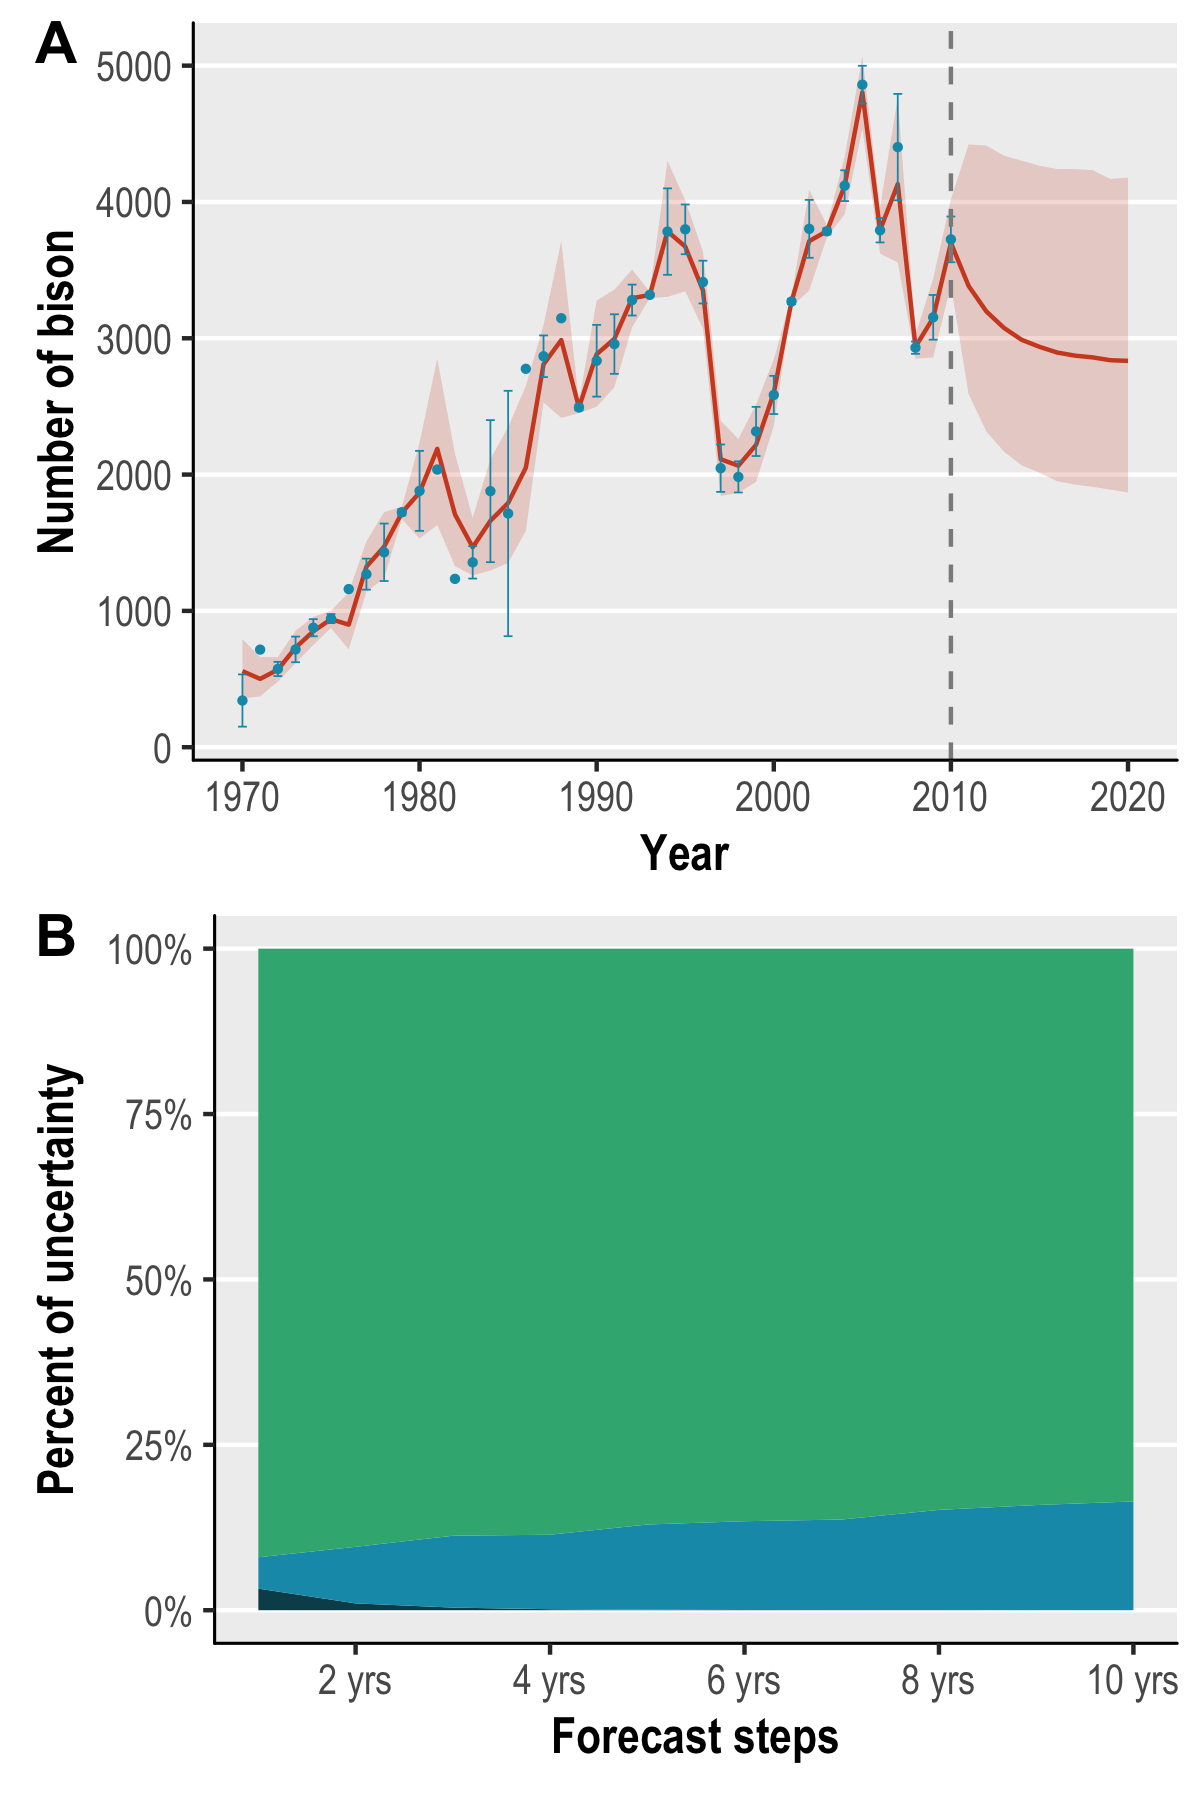
\includegraphics[height=4in]{../figures/bison_combined.png}
  \caption{An example state space model fit and forecast (A) and example of forecast uncertainty partitioning (B). In (A), points are observed counts and errorbars show the observed standard deviation; solid line is the median of the posterior distribution of the number of bison in Yellowstone and shaded area shows the 0.025 and 0.975 quantiles from the posterior distribution. Within-sample estimates are constrained by data, whereas the forecasts (past 2010) are not. Panel (B) shows the relative contribution of each source of forecast uncertainty over time.}
\end{wrapfigure}

where \(y_t\) is the observed state at time \emph{t}, \(z_t\) is the
latent state at time \emph{t}, \(\mu_t\) is the determinstic prediction
of the state at time \emph{t} given estimated parameters
(\(\boldsymbol{\theta_p}\)) for the specified model function
{[}\emph{f()}{]}, the latent state \emph{z} at time \emph{t}-1, and
\textbf{x} is a vector of environmental covariates. The two error terms
represent observation error (\(\sigma_{obs.}\)) and process error
(\(\sigma_{proc.}\)). The model is \emph{dynamic} because the future
state (\(z_t\)) depends on the previous state (\(z_{t-1}\)). For
simplicity we show the data and process models (Eqs. 3 and 4,
respectively) with normal likelihoods, but these distributions will vary
depending on the particular data generating process (Hobbs \& Hooten
2015).

\subsubsection{An Example: Yellowstone Bison}

We used annual counts of the Yellowstone bison (\emph{Bison bison}) from 1975 to 2010 to fit a
population growth model using a state-space approach (Equations 3-5).
After fitting the model, we made annual forecasts for 10 years into the
future with all uncertainty propagated (Fig. 1A). We made those same
forecasts with (\emph{i}) just initial condition uncertainty,
(\emph{ii}) initial condition and parameter uncertainty, and
(\emph{iii}) initial condition, parameter, and process uncertainty. This
set of forecasts allows us to partition the relative variance of
different sources, taking a numerical approach that is analagous to the
analytical approach shown in Equation 2.

The key result is that process uncertainty dominates forecast
uncertainty at all horizons (Fig. 1B). Initial condition
uncertainty decays very quickly, indicating strong internal population
regulation and the lack of chaotic dynamics, which is consistent with
our \textbf{Hypothesis H1}. The next step in testing \textbf{H1} is to
compare Fig. 1B to results from fast-growing populations.

\section{Participants}

We have assembled a diverse working group, with gender and career stage
diversity (Table 2). Of the 12 listed participants, four are women and
five are early career scientists. The proposed Powell Center Fellow is
Andrew Tredennick.

\footnotesize

\begin{longtable}[]{@{}llll@{}}
\caption{List of participants.}\tabularnewline
\toprule
\begin{minipage}[b]{0.22\columnwidth}\raggedright\strut
Name\strut
\end{minipage} & \begin{minipage}[b]{0.22\columnwidth}\raggedright\strut
Affiliation\strut
\end{minipage} & \begin{minipage}[b]{0.25\columnwidth}\raggedright\strut
Expertise\strut
\end{minipage} & \begin{minipage}[b]{0.19\columnwidth}\raggedright\strut
Associated Data set\strut
\end{minipage}\tabularnewline
\midrule
\endfirsthead
\toprule
\begin{minipage}[b]{0.22\columnwidth}\raggedright\strut
Name\strut
\end{minipage} & \begin{minipage}[b]{0.22\columnwidth}\raggedright\strut
Affiliation\strut
\end{minipage} & \begin{minipage}[b]{0.25\columnwidth}\raggedright\strut
Expertise\strut
\end{minipage} & \begin{minipage}[b]{0.19\columnwidth}\raggedright\strut
Associated Data set\strut
\end{minipage}\tabularnewline
\midrule
\endhead
\begin{minipage}[t]{0.22\columnwidth}\raggedright\strut
Andrew Tredennick*\(^{1,2,3}\)\strut
\end{minipage} & \begin{minipage}[t]{0.22\columnwidth}\raggedright\strut
Utah State University\\
\strut
\end{minipage} & \begin{minipage}[t]{0.25\columnwidth}\raggedright\strut
Data management/synthesis,\\
population forecasting\strut
\end{minipage} & \begin{minipage}[t]{0.19\columnwidth}\raggedright\strut
n/a\strut
\end{minipage}\tabularnewline
\begin{minipage}[t]{0.22\columnwidth}\raggedright\strut
Mevin Hooten*\(^\dagger\)\strut
\end{minipage} & \begin{minipage}[t]{0.22\columnwidth}\raggedright\strut
U.S. Geological Survey\\
\strut
\end{minipage} & \begin{minipage}[t]{0.25\columnwidth}\raggedright\strut
Bayesian modeling,\\
statistical forecasting\strut
\end{minipage} & \begin{minipage}[t]{0.19\columnwidth}\raggedright\strut
Sea otter\strut
\end{minipage}\tabularnewline
\begin{minipage}[t]{0.22\columnwidth}\raggedright\strut
Peter Adler*\strut
\end{minipage} & \begin{minipage}[t]{0.22\columnwidth}\raggedright\strut
Utah State University\\
\strut
\end{minipage} & \begin{minipage}[t]{0.25\columnwidth}\raggedright\strut
population ecology/modeling,\\
data synthesis\strut
\end{minipage} & \begin{minipage}[t]{0.19\columnwidth}\raggedright\strut
Idaho sagebrush\strut
\end{minipage}\tabularnewline
\begin{minipage}[t]{0.22\columnwidth}\raggedright\strut
Lauren Buckley*\strut
\end{minipage} & \begin{minipage}[t]{0.22\columnwidth}\raggedright\strut
University of Washington\\
\strut
\end{minipage} & \begin{minipage}[t]{0.25\columnwidth}\raggedright\strut
ecological forecasting\\
climate change\strut
\end{minipage} & \begin{minipage}[t]{0.19\columnwidth}\raggedright\strut
Grasshopper spp.\strut
\end{minipage}\tabularnewline
\begin{minipage}[t]{0.22\columnwidth}\raggedright\strut
Michael Dietze*\strut
\end{minipage} & \begin{minipage}[t]{0.22\columnwidth}\raggedright\strut
Boston University\\
\strut
\end{minipage} & \begin{minipage}[t]{0.25\columnwidth}\raggedright\strut
ecological forecasting,\\
partitioning uncertainty\strut
\end{minipage} & \begin{minipage}[t]{0.19\columnwidth}\raggedright\strut
n/a\strut
\end{minipage}\tabularnewline
\begin{minipage}[t]{0.22\columnwidth}\raggedright\strut
George Esslinger*\strut
\end{minipage} & \begin{minipage}[t]{0.22\columnwidth}\raggedright\strut
U.S. Geological Survey\\
Alaska Science Center\strut
\end{minipage} & \begin{minipage}[t]{0.25\columnwidth}\raggedright\strut
population monitoring,\\
GIS analysis\strut
\end{minipage} & \begin{minipage}[t]{0.19\columnwidth}\raggedright\strut
Sea otter\strut
\end{minipage}\tabularnewline
\begin{minipage}[t]{0.22\columnwidth}\raggedright\strut
Emily Farrer*\strut
\end{minipage} & \begin{minipage}[t]{0.22\columnwidth}\raggedright\strut
Tulane University\\
\strut
\end{minipage} & \begin{minipage}[t]{0.25\columnwidth}\raggedright\strut
population modeling,\\
Bayesian analysis\strut
\end{minipage} & \begin{minipage}[t]{0.19\columnwidth}\raggedright\strut
Niwot plants\strut
\end{minipage}\tabularnewline
\begin{minipage}[t]{0.22\columnwidth}\raggedright\strut
Jennifer Gremer*\strut
\end{minipage} & \begin{minipage}[t]{0.22\columnwidth}\raggedright\strut
University of California,\\
Davis\strut
\end{minipage} & \begin{minipage}[t]{0.25\columnwidth}\raggedright\strut
plant population modeling\\
data management\strut
\end{minipage} & \begin{minipage}[t]{0.19\columnwidth}\raggedright\strut
Winter annuals\strut
\end{minipage}\tabularnewline
\begin{minipage}[t]{0.22\columnwidth}\raggedright\strut
Janneke HillRisLambers*\strut
\end{minipage} & \begin{minipage}[t]{0.22\columnwidth}\raggedright\strut
University of Washington\strut
\end{minipage} & \begin{minipage}[t]{0.25\columnwidth}\raggedright\strut
plant population modeling,\\
climate change\strut
\end{minipage} & \begin{minipage}[t]{0.19\columnwidth}\raggedright\strut
Mt. St.~Helens plants\strut
\end{minipage}\tabularnewline
\begin{minipage}[t]{0.22\columnwidth}\raggedright\strut
N. Thompson Hobbs*\(^\dagger\)\strut
\end{minipage} & \begin{minipage}[t]{0.22\columnwidth}\raggedright\strut
Colorado State University\\
\strut
\end{minipage} & \begin{minipage}[t]{0.25\columnwidth}\raggedright\strut
population ecology,\\
state space models\strut
\end{minipage} & \begin{minipage}[t]{0.19\columnwidth}\raggedright\strut
Yellowstone bison\strut
\end{minipage}\tabularnewline
\begin{minipage}[t]{0.22\columnwidth}\raggedright\strut
Ethan White*\strut
\end{minipage} & \begin{minipage}[t]{0.22\columnwidth}\raggedright\strut
University of Florida\\
\strut
\end{minipage} & \begin{minipage}[t]{0.25\columnwidth}\raggedright\strut
ecological forecasting,\\
data synthesis\strut
\end{minipage} & \begin{minipage}[t]{0.19\columnwidth}\raggedright\strut
BBS \& Portal Data\strut
\end{minipage}\tabularnewline
\begin{minipage}[t]{0.22\columnwidth}\raggedright\strut
Perry Williams*\(^\dagger\)\strut
\end{minipage} & \begin{minipage}[t]{0.22\columnwidth}\raggedright\strut
Colorado State University\\
\strut
\end{minipage} & \begin{minipage}[t]{0.25\columnwidth}\raggedright\strut
spatiotemporal modeling,\\
population forecasts\strut
\end{minipage} & \begin{minipage}[t]{0.19\columnwidth}\raggedright\strut
Sea otter\strut
\end{minipage}\tabularnewline
\bottomrule
\end{longtable}

\vspace{-2em}

*Confirmed participant\\
\(^\dagger\)Local (Ft. Collins) participant\\
\(^1\)Powell Center Fellow\\
\(^2\)Technical liaison to Powell Center computing staff\\
\(^3\)Party responsible for adherence to Powell Center Data and
Information Policy

\normalsize

\section{Time Table of Activities}\begin{description}

\item[October to December 2017] Monthly PI Skype meetings to prepare for first meeting. Begin email exchanges to confirm participants. Write \texttt{R} scripts to download, clean, and aggregate data.
\item[January 2018] \textit{First meeting at Powell Center}: Identify other appropriate data sets. Decide on model structures for each data set and identify environmental covariates. Form two-person analysis teams for each data set. Go through bison analysis example. Define manuscripts.
\item[February to December 2018] Bi-monthly PI Skype meetings. Continue and finalize data set acquisition and aggregate into single database for analysis teams. Analysis teams, with the PC Fellow, identify appropriate environmental drivers for their system and begin fitting models. PC Fellow writes generalizable \texttt{R} functions for analysis teams. PC Fellow has Skype meetings with each analysis team as needed to complete analyses. Write first drafts of manuscripts.
\item[January 2019] \textit{Second meeting at Powell Center}: Analysis teams present results for feedback. Finalize database and identify any outstanding issues. Evaluate manuscript drafts and form writing teams. Create a \textsc{GitHub} repository for forecasts.
\item[February to June 2019] Finalize database and forecast repository. Finalize all forecasts and forecast partitions. Continue writing manuscripts. PC Fellow will have at least one Skype meeting with each analysis team during this period.
\item[July to September 2019] Complete manuscripts and submit for publication. Release database and forecast repository to Powell Center for permanent archiving. In addition to peer-reviewed papers, write a blog post for Dynamic Ecology\footnote{http://dynamicecology.wordpress.com/} on the limits to ecological forecasting to reach an even broader audience.

\end{description}

\section{Anticipated Results and Benefits}

The greatest benefit of this project will be the conceptual advance of
linking ecological theory to sources of forecast uncertainty. We
anticipate that research associated with this project will catalyze a
new area of research on ecological forecasting. The working group
participants will gain experience using cutting-edge quantitative
techniques. The assembled database of plant and animal abundance time
series, coupled with environmental covariates, will be a valuable
resource for teaching and research, and the repository of population
forecasts will provide new opportunities to validate, and improve,
forecasts. No repository of ecological forecasts currently exists, but
one of our participants (M. Dietze) plans to develop one as part of the
NSF-funded \emph{Near-term Ecological Forecasting Initiative}. Our
working group and his project will work synergistically to create a
repository. In addition, we expect to produce several publications,
including:

\begin{enumerate}
\def\labelenumi{\arabic{enumi}.}
\tightlist
\item
  A synthesis paper testing our hypotheses using all the data sets aimed
  at \emph{PNAS} or \emph{Ecology Letters}.
\item
  A forum-style paper on the limits to ecological forecasting, how to
  overcome them, and the usefulness of even uncertain forecasts for
  ecosystem management for \emph{Frontiers in Ecology and the
  Environment}.
\item
  Several in-depth papers on forecasts of specific populations aimed at
  top-tier applied journals such as \emph{Ecological Applications} and
  \emph{Journal of Applied Ecology}.
\end{enumerate}

\section{Literature Cited}\label{references}
\addcontentsline{toc}{section}{References}

\hypertarget{refs}{}
\hypertarget{ref-Bauer2015}{}
Bauer, P., Thorpe, A. \& Brunet, G. (2015). The quiet revolution of
numerical weather prediction. \emph{Nature}, 525, 47--55.

\hypertarget{ref-Botero2015}{}
Botero, C.A., Weissing, F.J., Wright, J. \& Rubenstein, D.R. (2015).
Evolutionary tipping points in the capacity to adapt to environmental
change. \emph{Proceedings of the National Academy of Sciences}, 112,
184--189.

\hypertarget{ref-Clark2001}{}
Clark, J.S., Carpenter, S.R., Barber, M., Collins, S., Dobson, A.,
Foley, J.A., et al. (2001). Ecological forecasts: an emerging
imperative. \emph{Science}, 293, 657--660.

\hypertarget{ref-DelMoral2010}{}
{del Moral}, R. (2010). Thirty years of permanent vegetation plots,
Mount St. Helens, Washington, USA. \emph{Ecology}, 91, 2185.

\hypertarget{ref-Dietze2017}{}
Dietze, M. (2017). \emph{Ecological Forecasting}. Princeton University
Press, Princeton.

\hypertarget{ref-Gremer2014}{}
Gremer, J.R. \& Venable, D.L. (2014). Bet hedging in desert winter
annual plants: Optimal germination strategies in a variable environment.
\emph{Ecology Letters}, 17, 380--387.

\hypertarget{ref-Hobbs2015}{}
Hobbs, N.T. \& Hooten, M.B. (2015). \emph{Bayesian Models: A Statistical
Primer for Ecologists}. Princeton University Press, Princeton.

\hypertarget{ref-Hobbs2015EcolMon}{}
Hobbs, N.T., Geremia, C., Treanor, J., Wallen, R., White, P.J., Hooten,
M.B., et al. (2015). State-space modeling to support management of
brucellosis in the Yellowstone bison population. \emph{Ecological
Monographs}, 85, 525--556.

\hypertarget{ref-Houlahan2017}{}
Houlahan, J.E., Mckinney, S.T., Anderson, T.M. \& Mcgill, B.J. (2017).
The priority of prediction in ecological understanding. \emph{Oikos},
126, 1--7.

\hypertarget{ref-Petchey2015}{}
Petchey, O.L., Pontarp, M., Massie, T.M., Kéfi, S., Ozgul, A.,
Weilenmann, M., et al. (2015). The ecological forecast horizon, and
examples of its uses and determinants. \emph{Ecology Letters}, 18,
597--611.

\hypertarget{ref-Steffen2015}{}
Steffen, W., Richardson, K., Rockström, J., Cornell, S., Fetzer, I.,
Bennett, E., et al. (2015). Planetary boundaries: Guiding human
development on a changing planet. \emph{Science}, 348, 1217.

\hypertarget{ref-Tredennick2016MEE}{}
Tredennick, A.T., Hooten, M.B. \& Adler, P.B. (2016a). Do we need
demographic data to forecast plant population dynamics? \emph{Methods in
Ecology and Evolution}, n/a--n/a.

\hypertarget{ref-Tredennick2016Ecos}{}
Tredennick, A.T., Hooten, M.B., Aldridge, C.L., Homer, C.G.,
Kleinhesselink, A.R. \& Adler, P.B. (2016b). Forecasting climate change
impacts on plant populations over large spatial extents.
\emph{Ecosphere}, 7, e01525.

\hypertarget{ref-Williams2017}{}
Williams, P.J., Hooten, M.B., Womble, J.N., Esslinger, G.G., Bower, M.R.
\& Hefley, T.J. (2017). An integrated data model to estimate
spatio-temporal occupancy, abundance, and colonization dynamics.
\emph{Ecology}, 0, 1--9.


\end{document}
